\documentclass{beamer}

\mode<presentation>
{
\usetheme{Darmstadt}%Darmstadt,Frankfurt

\setbeamercovered{transparent}
}
%Deutsche Silbentrennung
\usepackage[ngerman]{babel}
%Deutsche Umlaute
\usepackage[utf8]{inputenc}
%Listen einr�cken
\usepackage{enumitem}
% font definitions, try \usepackage{ae} instead of the following
% three lines if you don't like this look
\usepackage{mathptmx}
\usepackage[scaled=.90]{helvet}
\usepackage{courier}
%Trennung von deutschen Umlauten
\usepackage[T1]{fontenc}
\usepackage{adjustbox}

\title{Sicherheit in Android und iOS}

%\subtitle{}

% - Use the \inst{?} command only if the authors have different
%   affiliation.
%\author{F.~Author\inst{1} \and S.~Another\inst{2}}
\author{David Artmann\inst{1} \and Kristoffer Schneider\inst{1}}

% - Use the \inst command only if there are several affiliations.
\institute[Universities of]
{
\inst{1}
Hochschule für angewandte Wissenschaften\\
Würzburg-Schweinfurt
}

\date{\today}


% This is only inserted into the PDF information catalog. Can be left
% out.
\subject{Talks}



% If you have a file called "university-logo-filename.xxx", where xxx
% is a graphic format that can be processed by latex or pdflatex,
% resp., then you can add a logo as follows:
\pgfdeclareimage[height=0.5cm]{university-logo}{media/logo/fhws.png}
\logo{\pgfuseimage{university-logo}}



% Delete this, if you do not want the table of contents to pop up at
% the beginning of each subsection:
\AtBeginSubsection[]
{
\begin{frame}<beamer>
\frametitle{Gliederung}
\tableofcontents[currentsection,currentsubsection]
\end{frame}
}

% If you wish to uncover everything in a step-wise fashion, uncomment
% the following command:
\beamerdefaultoverlayspecification{<+->}

\begin{document}

% titlepage
\begin{titlepage}
	%Eine mbox wird verwendet um Text zusammenzuhalten
	%vspace erzeugte die in Klammern angegebenen Zeilenabstände
	%baselineskip setzt zeilenabstand
   	\mbox{}\vspace{5\baselineskip}\\
   	%Schriftart und Größe als Attribut
   	\rmfamily\huge
   	%Mittige Textausrichtung (\centerline für eine Zeile)
   	\centering
   	%Das Argument erscheint in Kapitaelchen (small capitals).
	\textsc{Sicherheit in Android und iOS}
	%Umbruch bezogen auf die Hoehe des Kleinbuchstaben x in diesem Element * Faktor
	\\[3ex]
   	Seminararbeit
   	\rmfamily\Large
   	\vspace{1\baselineskip}\\
   	%Externes einbinden einer Textdatei
   	%% versionsnummer entfernt
   	%\input{version.txt}\mbox{}
	\vspace{3\baselineskip}
	Hochschule für angewandte Wissenschaften Würzburg-Schweinfurt
   	\vspace{5\baselineskip}\\
   	\rmfamily\Large
   	David Artmann\\
   	\rmfamily\Large
   	Kristoffer Schneider
   	\vspace{1\baselineskip}\\
   	%Heutiges Datum
   	\today
\end{titlepage}

% toc
\begin{frame}
	\frametitle{Gliederung}
	\tableofcontents
	% You might wish to add the option [pausesections]
\end{frame}


\section{Gemeinsamkeiten und Unterschiede}
	\subsection[Systemsicherheit]{Systemsicherheit}
		\section{Komponenten der Systemsicherheit unter
iOS}\label{sec:components-syssec} 
	Eine Kette von aneinander gereihten und von einander abhängigen Prozessen trägt
	maßgeblich zur Systemsicherheit von iOS bei. Dies berücksichtigt vor allem den
	Startvorgang, die Softwareupdates - auch von Drittanbietern - und den Secure
	Enclave (Kapitel \ref{sec:secure_enclave}). Dies stellt sicher, dass
	alle Kernkomponenten, ob Hard- oder Software, möglichst gefeit vor Angriffen sind,
	ohne dabei die Nutzerfreundlichkeit zu beeinflussen. Wenn dabei einer dieser
	Schritte fehlschlägt, unterbricht der Startvorgang und das Gerät wird in den
	Recovery Modus versetzt. Wenn der Boot-ROM nicht geladen werden kann, wird der
	DFU\footnote{Device Firmware Upgrade: DFU} Modus
	betreten.\\
	Nachfolgend werden die Komponenten, welche maßgeblich zur Wahrung der
	Systemsicherheit und der Integrität dieser beteiligt sind, detailliert
	vorgestellt und beschrieben.
	
	\begin{figure}[h]
		\centering
		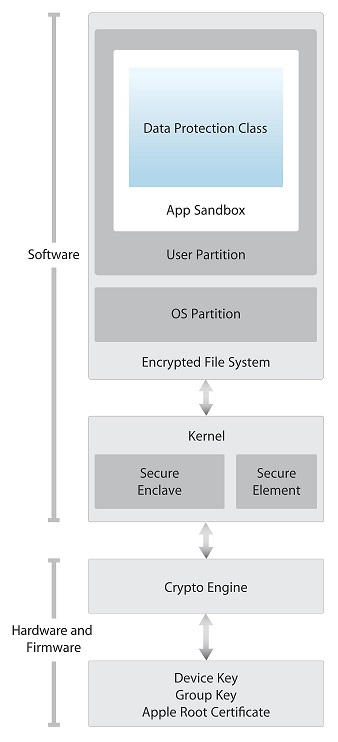
\includegraphics[width=0.4\linewidth]{ios/media/security-model.jpg}
		\caption{Sicherheitsmodel von iOS 
		\cite[S.4]{iOSSecurityApr2015}}
		\label{fig:security-model}
	\end{figure}

	%TODO: look at learning ios security, there this whole process is explained
	% good
	\subsection{Secure boot chain}\label{sec:secure-boot-chain}
		Dieses Verfahren stellt eine Manipulation der Low-Level Software sicher. Nur
		iOS Geräte, deren Vertrauenskette erfolgreich validiert wurde, starten
		ordnungsgemäß. Dabei wird nach dem Start eines iOS Gerätes zuerst Code aus
		einem nur lesbaren Speicherbereich ausgeführt. Dieser \textit{hardware of
		trust} genannte und unveränderbare Code ist bei der Manufaktur der Chips
		eingebettet worden und somit implizit vertraulich. Das Boot ROM enthält
		zusätzlich den öffentlichen Schlüssel der Wurzel Zertifizierungsstelle von
		Apple, welcher eine Signierung des Low-Level-Bootloaders durch Apple sicher
		stellt, bevor er ausgeführt wird.
		Dies ist der erste Schritt in der "`chain of trust"', in welcher jeder
		Teilnehmer sicher stellt, dass der darauf folgende von Apple signiert ist. 		
		Nach erfolgreicher Abarbeitung aller Aufgaben des LLB, überprüft und startet
		dieser iBoot, den nächsten Bootloader, welcher wiederrum das selbe Prozedere
		mit dem iOS Kernel beginnt. Bei Geräten mit Mobilfunk Zugang führt das
		Basisband Untersystem seinen eigenen ähnlichen Prozess mit signierter 
		Software und verifizierten Schlüsseln des Basisband Prozessors durch.
		
	\subsection{Authorisierung von System Software}\label{sec:code-signing}
		Dieser Prozess soll einen Downgrade auf eine ältere Version von iOS
		verhindern. Der im folgenden Kapitel besprochene Secure Enclave Co-Prozessor
		nutzt diese Technik für Integritätsprüfung seiner Software ebenfalls. Im Falle
		eines iOS Updates wird entweder von iTunes oder vom Gerät selbst einer der
		autorisierenden Installationsserver von Apple kontaktiert. Diesem
		wird eine Liste von verschlüsselten Informationen pro am Update beteiligter
		Komponente gesandt. Zusätzlich wird ein zufälliger
		%TODO: add long version of ECID
		Anti-Replay Wert und die eindeutige ID des Gerätes
		verschickt. Die Clientdaten werden gegen eine Auflistung authorisierter Hardware, für die ein
		Update genehmigt sind geprüft. Bei Übereinstimmung wird die
		ECID\footnote{Eindeutige ID: ECID} zu den Informationen hinzugefügt und das
		Ergebnis signiert, was einer Personalisierung der Daten gleicht.
		Anschließend werden alle nötigen Daten vom Server signiert und zum Gerät
		geschickt. Die sichere Startkette von Prozessen (Kapitel
		\ref{sec:secure-boot-chain}) verifiziert die Signatur der empfangenen Daten
		auf den Absender Apple und gleicht die Prüfsumme der Signatur mit dem lokalen
		Ergebnis von verschlüsselten Informationen und ECID ab.\\
		Mit diesen Schritten wird eine Authorisierung ausschließlich für authorisierte
		Geräte sicher gestellt. Außerdem verhindert der Anti-Replay Wert ein
		Manipulieren der Serverdaten, oder ein Mitschneiden dieser für
		das Verwenden auf anderen, nicht authorisierten Geräten.
	\subsection{Secure Enclave}\label{sec:secure_enclave}
		%TODO: get more details for ensuring the facts in this chapter
		Dieser Co-Prozessor kommt in Geräten mit A7 oder jüngeren A-Serien Prozessoren
		vor. Er verwendet seinen eigenen sicheren Startvorgang, ist separiert vom
		Applikations Prozessor und verwendet verschlüsselten Speicher, sowie einen
		Hardware Zufallszahlen Generator. Die Technologie basiert auf ARM's
		TrustZone\cite{TrustZone2015}
		und wurde von Apple für die eigenen Ansprüche angepasst. Der Kernel dieser
		Einheit basiert auf der L4
		Mikrokernel-Familie\cite{L4MicroKernel2015} mit leichten
		Modifikationen. Die auf Interrupts basierende Kommunikation zwischen dem
		Applikationsprozessor und dem Secure Enclave läuft über einem nur den beiden zur Verfügung stehenden Speicherbereich.
		Der SE\footnote{SE: Secure Enclave} ist verantwortlich für das Schlüssel
		Management der Datenverschlüsselung und stellt die Integrität dieser sicher, auch wenn der
		Kernel des iOS Systems kompromitiert ist. Beim Herstellungsprozess erhält
		jeder SE eine einzigartige ID, auf welche nur er zugreifen kann. Selbst Apple,
		oder anderen an der Produktionskette beteiligten Herstellern ist diese nicht bekannt.
		Mit dieser UID\footnote{Einzigartige ID: UID} wird beim Systemstart der
		Speicherbereich des SE zusammen mit einem einmaligen Schlüssel verschlüsselt.
		Zusätzlich werden jegliche vom SE in den Speicher geschriebene Daten mit der
		UID und einem Anti-Replay Zufallswert verschlüsselt. Eine der Hauptaufgaben
		des Secure Enclave ist die verarbeitung der Fingerabdruck-Daten des Touch ID
		(Kapitel \ref{sec:touch_id}).
		Alle Kommunikation zwischen Touch ID und SE wird über einen seriellen Bus
		abgearbeitet. Der Applikationsprozessor leitet die Fingerabdrucksdaten an den
		SE weiter kann diese aber aufgrund einer Verschlüsselung der Daten mit einem
		Sitzungsschlüssel nicht lesen. Dieser Session Key wurde durch den für Touch
		ID und SE bereit gestellten öffentlichen Schlüssel erzeugt. Der Austausch des
		%TODO: long form of AES in footmark
		Sitzungsschlüssels wird durch AES Key Wrapping realisiert. Dabei erzeugen
		beide Seiten einen zufälligen Schlüssel, welche den Sitzungsschlüssel bilden.
		%TODO: long form of AES-CCM in footmark
		Zum verschlüsselten Transport wird AES-CCM genutzt.
	\subsection{Touch ID}\label{sec:touch_id}
		Touch ID bezeichnet den Fingerabdrucksensor der in allen iPhone 5s und neuer
		, sowie iPad Air 2 und iPad mini 3 verbaut ist. Es können bis zu 5
		%TODO: check if advantage is the locking or maybe ENCRYPTION, when s/w-button
		% is pressed
		Fingerabdrücke gespeichert werden. Eine der größten Vorteile dabei ist das
		sofortige Sperren des Gerätes beim drücken des Sleep/Wake-Buttons. Dies gilt
		auch bei aktiviertem Passcode. Vor der Einführung von Touch ID haben viele
		%TODO: details of Passcode in footmark, or in sentence after mention it?
		Nutzer eine möglichst lange Zeit eingestellt, bis das Eingeben des Passcodes
		nötig wurde, nachdem das Gerät gesperrt wurde. Dies entfällt nun bei
		aktivierter Touch ID, da der Nutzer nur noch mit seinem Finger Entsperren
		muss.
		Touch ID kann zusätzlich zum Entsperren des Gerätes auch mit dem Zahlungsdienst Apple
		Pay und für Einkäufe in iTunes, dem App Store und im iBook Store genutzt
		werden. Für Entwickler steht eine API bereit mit der rudimentärste
		Prüfungen auf erfolgreiche Verifikation des Abdrucks erfolgen können. Ein
		direkter Zugriff auf Touch ID oder die Daten des Fingerabdrucks wird von
		Apple unterbunden. Touch ID wird aktiviert, wenn der kapazitive Stahlring um
		den Sensor einen Fingerdruck wahrnimmt. Anschließend wird dieser gescannt und
		an den Secure Enclave gesandt. Der Abdruck wird kurzzeitig im veschlüsselten
		%TODO: better description?!
		Speicher des SE für eine Vektorisierung der Fingerabdruckdaten gespeichert, um
		danach verworfen zu werden. Die Schlüssel, welche von Touch ID zum
		Entschlüsseln des Gerätes benötigt werden, sind nach 48 Stunden ungültig,
		beziehungsweise wenn das iOS Gerät neu gestartet wurde, oder der
		Fingerabdruck fünf mal falsch registriert wurde.\\
		Dass diese Technik nicht als Sicher angesehen werden darf, haben bereits
		Miglieder des Chaos Computer Club gezeigt\cite{CCCBreakTouch2015}, dabei 
		wurde mit simpelsten Haushaltsmitteln ein Fingerabdruck gefälscht, den das
		Smartphone irrtümlicher weise akzeptiert hat.

		%% grober aufbau ist sehr ähnlich, siehe:
		%hardware (TEE, SE)
		%bootvorgang (secure boot chain)
		%userland (sandboxing, rechte)
	\subsection[Applikationssicherheit]{Applikationssicherheit}
		\begin{frame}

	\begin{block}{}
		App-Berechtigungen
	\end{block}
	\begin{itemize}
	  \item iOS bis Android M granularer
	  \item Zeitweise Abhilfe durch AppOps
	  \item Mit iOS 9 und Android M gleichauf
	\end{itemize}
	
	\begin{block}{}
		App-Distribution
	\end{block}
	\begin{itemize}
	  \item iOS nur über Apple's App Store
	  \item Android bietet diverse (Google Play, F-Droid, Amazon App-Shop)
	\end{itemize}

\end{frame}
		\begin{frame}

	\centering
	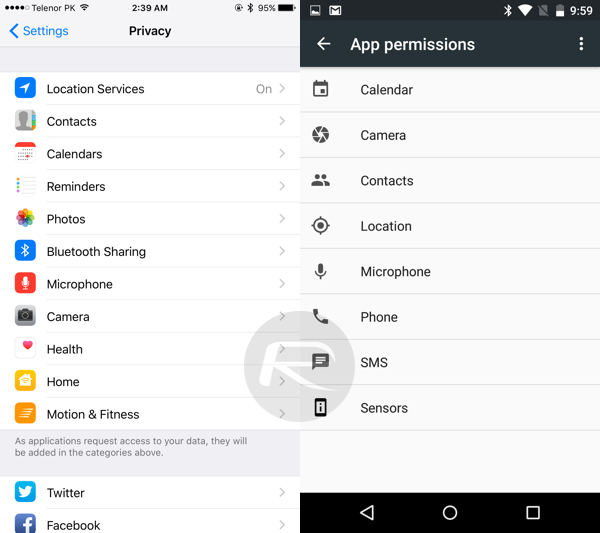
\includegraphics[height=0.5\linewidth]{media/graphics/ios-9-vs-android_privacy.png}

%\begin{columns}[T] % contents are top vertically aligned
%	\begin{column}[T]{5cm} % each column can also be its own environment
%		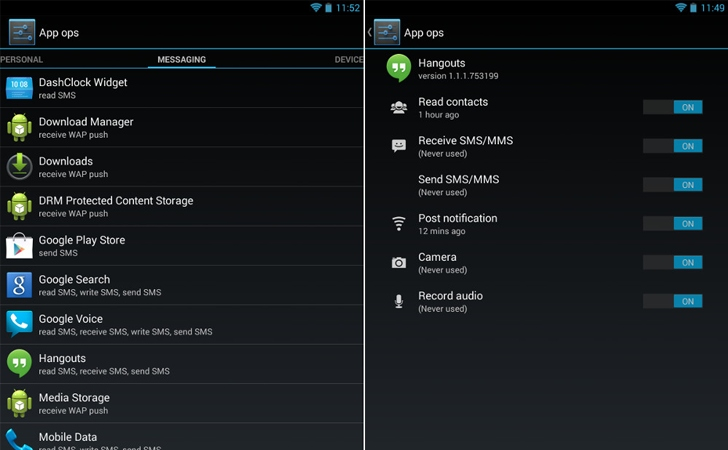
\includegraphics[height=3cm]{media/graphics/appops-android.jpg}
%	\end{column}
%	\begin{column}[T]{5cm} % alternative top-align that's better for graphics
%    	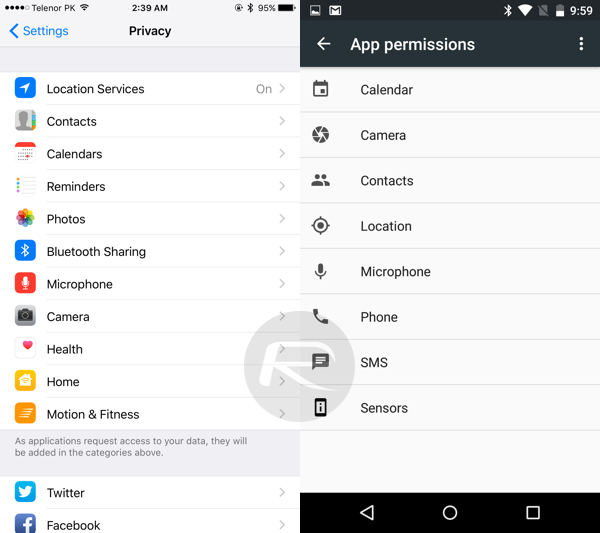
\includegraphics[height=3cm]{media/graphics/ios-9-vs-android_privacy.png}
%	\end{column}
%\end{columns}

\end{frame}
		%% unterschiede liegen im detail, siehe:
		%unterschied bei TEE und SE
		%benutzerrechtesystem intern mit linux+unix usern
		%berechtigungen der apps android vs. ios (alles oder nichts)
		
		
\section{Systemkultur}
	\subsection{Android vs. iOS}
		\begin{frame}
\frametitle{Systemkultur}
\framesubtitle{}
	\center{Android vs. iOS}\\
	\textsl{Hier soll der direkte Vergleich von Android vs. iOS erscheinen}
	\begin{table}
		%TODO
	\end{table}
\end{frame}
	\subsection{Opensource von Android}
	\subsection{Proprietät unter iOS}
		\begin{frame}

	\center{
\includegraphics[height=0.2\linewidth]{media/graphics/Apple_logo_black.png}}
	\begin{block}{}
		Produktion HW/SW im eigenen Haus
	\end{block}
	\begin{block}{}
		Ungewissheit durch Proprietät
	\end{block}
	\begin{block}{}
		Umgehen dieser Politik durch Jailbreaking
	\end{block}

\end{frame}
		\begin{frame}
	\centering
	\textbf{Historische Exploits}
	\begin{columns}[T] % contents are top vertically aligned
    	\begin{column}[T]{5cm} % each column can also be its own environment
    		\begin{block}{}
				libTiff Exploit
			\end{block}
			\begin{block}{}
				Ikee Virus
			\end{block}
			\begin{block}{}
				SpyPhone
			\end{block}
    	\end{column}
	\end{columns}

\end{frame}
		\begin{frame}
	\centering
	\textbf{lockdownd}
	\begin{block}{}
		Ermöglicht Zugriff über TCP Port 62078
	\end{block}
	\begin{block}{}
		Abarbeitung über eigenes Protokoll \textsl{usbmux}
	\end{block}
	\begin{block}{}
		Übergebene Portnummer auf localhost
	\end{block}

\end{frame}
		\begin{frame}
	\centering
	com.apple.mobile.\textbf{pcapd}
	\begin{block}{}
		Sniffingsoftware auf Basis von \textsl{pcap}
	\end{block}
	\begin{block}{}
		Implementierung durch Bibliothek \textsl{libcap}
	\end{block}
	\begin{block}{}
		Kein visueller Hinweis auf Aktivität des Dienstes
	\end{block}
	\begin{block}{}
		Seit iOS 8 nicht mehr über WLAN ansprechbar
	\end{block}
\end{frame}
		\begin{frame}
	\centering
	com.apple.mobile.\textbf{file\_relay}
	\begin{block}{}
		Zugriff auf Adressbuch, GPS Daten, Fotos
	\end{block}
	\begin{block}{}
		Metadaten Abbild des Dateisystems
	\end{block}
	\begin{block}{}
		Apple:
		\begin{quote}
			In iOS 8 and later, this capability requires additional configuration before
			use.
		\end{quote}
	\end{block}
\end{frame}
		\begin{frame}
	\centering
	com.apple.mobile.\textbf{house\_arrest}
	\begin{block}{}
		Offiziell für Datentransfer von iTunes und Testdaten für Xcode
	\end{block}
	\begin{block}{}
		Zdziarski: Zugriff auf Library, Cache, Cookies, bevorzugte Ordner
	\end{block}
	\begin{block}{}
		Obwohl die iTunes GUI dies nicht erlaubt
	\end{block}
\end{frame}
		\begin{frame}
	\centering
	\textbf{Historische Exploits}
	\begin{columns}[T] % contents are top vertically aligned
    	\begin{column}[T]{5cm} % each column can also be its own environment
    		\begin{block}{}
				libTiff Exploit
			\end{block}
			\begin{block}{}
				Ikee Virus
			\end{block}
			\begin{block}{}
				SpyPhone
			\end{block}
    	\end{column}
	\end{columns}

\end{frame}
		\begin{frame}
	\centering
	\textbf{libTiff Exploit} (2007)
	\begin{block}{}
		Pufferüberlauf der libtiff Bibliothek
	\end{block}
	\begin{block}{}
		Wurde für Jailbreak genutzt
	\end{block}
	\begin{block}{}
		iOS Prozesse liefen noch mit root (iOS 1)
	\end{block}
\end{frame}
		\begin{frame}
	\centering
	\textbf{Ikee Virus}
	\begin{block}{}
		Einer der ersten Würmer unter iOS (2009)
	\end{block}
	\begin{block}{}
		Standardpasswort der Jailbreak SSH Zugänge ausgenutzt
	\end{block}
	\begin{block}{}
		Bösartige Variante \textsl{Ikee.B} stahl Daten
	\end{block}
\end{frame}
	%% opensource vs. proprietät
	%nachteile: Android: updateproblematik, transparenzprobleme(drittanbieter
	% eigenbauten) vorteile: closed source, proprietär
	%MDM/BYOD: iOS einfacher, Android komplex, schwieriger
	%% Systemmodifikation
	%android erlaubt das rooten, ios nicht (exploits: jailbreak)
	%Feststellen von Rooting unter Android sehr schwer, unter iOS relativ einfach
	% (fork())
	
\section{Härten}
	\subsection{Tips für Endnutzer}
	%% generelle tips
	%% spezifische tips
	\subsection{Ratschläge für Entwickler}
	%% generelle tips
	%
	%% spezifische tips
	

%\begin{frame}
%\frametitle{}

% You can create overlays
%\begin{itemize}
%  \item using the \texttt{pause} command:
%  \begin{itemize}
%    \item First item.
%    \pause
%    \item Second item.
%  \end{itemize}
%  \item using overlay specifications:
%  \begin{itemize}
%    \item<3-> First item.
%    \item<4-> Second item.
%  \end{itemize}
%  \item using the general \texttt{uncover} command:
%  \begin{itemize}
%    \uncover<5->{\item First item.}
%    \uncover<6->{\item Second item.}
%  \end{itemize}
%\end{itemize}
%\end{frame}

%\section*{Summary}

%\begin{frame}
%\frametitle<presentation>{Summary}

%\begin{itemize}
%  \item The \alert{first main message} of your talk in one or two lines.
%\end{itemize}

% The following outlook is optional.
%\vskip0pt plus.5fill
%\begin{itemize}
%  \item Outlook
%  \begin{itemize}
%    \item Something you haven't solved.
%    \item Something else you haven't solved.
%  \end{itemize}
%\end{itemize}
%\end{frame}

\end{document}
